\documentclass[a4paper,11pt]{article}

\usepackage[T1]{fontenc}
\usepackage[utf8]{inputenc}
\usepackage[english,polish]{babel}
\usepackage{lmodern}
\usepackage{graphicx}
\usepackage{fancyhdr}
\usepackage{float}
\usepackage{array}
%\usepackage{mathtools}


\setlength{\textheight}{23.5cm}
\setlength{\textwidth}{15.92cm}
\setlength{\footskip}{10mm}
\setlength{\oddsidemargin}{0mm}
\setlength{\evensidemargin}{0mm}
\setlength{\topmargin}{0mm}
\setlength{\headsep}{15mm}
\setlength{\parindent}{0cm}
\setlength{\parskip}{2.5mm}

\begin{document}


\begin{center}

    \begin{tabular}{ | m{5cm}| m{5cm} | m{5cm} |}
    \hline 
    \multicolumn{2}{|c|}{Elektronika w eksperymencie fizycznym}
    & Rok akademicki 2012-2013 \\ 
    
    \hline
    Środa 14.15-17.00 
    & Justyna Ilczuk \newline Jacek Rosiński
    & Wykonane w dniu 3.04.2013 \\
   	
   	\hline
   	Ćwiczenie 6 & Falowody i linie długie &    Ocena: \\
   	\hline
    \end{tabular}
\end{center}

%\newpage
\pagestyle{fancy}
\fancyfoot[CO]{\ }
\fancyhead[RO]{\footnotesize{\thepage} }
%\fancyhead[RO]{\footnotesize{\ } }
\fancyhead[LO]{Justyna Ilczuk i Jacek Rosiński K-1, Falowody i linie długie}





\section{Cel ćwiczenia}
Celem ćwiczenia było:
zapoznanie się z transmisją sygnałów elektrycznych w liniach długich i przeprowadzenie pomiarów: długości fali, współczynnika fali stojącej, współczynnika odbicia.

\section{Użyty sprzęt i układy pomiarowe}
W naszym ćwiczeniu używaliśmy trzech układów pomiarowych.

W części pierwszej mierzyliśmy fale decymetrowe. Najpierw zmierzyliśmy kolejne miejsca, w których wystąpił węzeł fali stojącej,
a potem po zmianie obciążenia na końcu linii, zmierzyliśmy wartość maksymalną i minimalną fali. 
Schemat układu do badania fal decymetrowych przedstawia poniższy rysunek: 

\begin{figure} [H]
  \begin{center}
    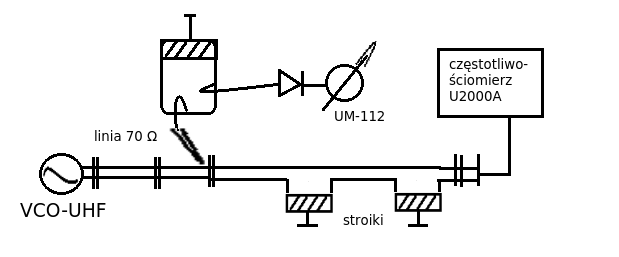
\includegraphics{Edecy.png}
  \end{center}
\end{figure}
VCO-UHF – generator fal decymetrowych.
Linia 70 $\Omega$  - odcinek linii dopasowującej.
Stroiki umożliwiają całkowite dopasowanie, co w rezultacie daje falę stojącą (w węzłach fali minimalne wartości).
Linia pomiarowa składa się z anteny sprzężonej z rezonatorem, elementy te umieszczone są na ruchomej karetce z odpowiednią skalą umożliwiającą pomiar odległości np. między węzłami fali stojącej. Antena poprzez cienki otwór w falowodzie umieszczona jest wewnątrz jego. Układ anteny i rezonatora połączony jest z detektorem, na wyjściu którego mierzone jest napięcie przez miernik UM-112.

W części drugiej mierzyliśmy fale centymetrowe w analagiczny sposób. Tym razem jednak posłużyliśmy się schematem z poniższego rysunku: 
\begin{figure} [H]
  \begin{center}
    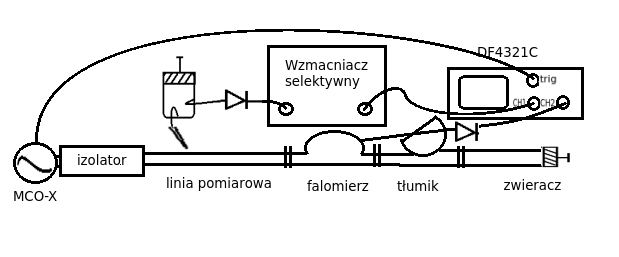
\includegraphics{Ecenty.png}
  \end{center}
\end{figure}
MCO-X – generator fal centymetrowych modulowanych przebiegiem prostokątnym o częstotliwości 1kHz
Izolator zapewnia tylko jeden kierunek fali zgodny ze strzałką, zapobiega to przesterowaniu generatora.
Tłumik – służy do tłumienia fali odbitej, zbudowany jest z układu ruchomych płytek nieprzepuszczalnych dla fal EM. Dzięki takiej budowie możliwa jest płynna regulacja tłumienia.

W części trzeciej ćwiczenia generowaliśmy impuls w linii długiej, sygnał wpuszczaliśmy jednocześnie do oscyloskopu i do długiego kabla bez obciążenia. Sygnał ulegał odbiciu w linii długiej i na oscyloskopie mogliśmy zaobserwować dwa impulsy przesunięte w czasie. W tej części zmierzyliśmy różnice czasów dla dwóch kabli i długość jednego kabla. Schematycznie nasz układ pomiarowy można przedstawić jak na rysunku pod spodem: 

\begin{figure} [H]
  \begin{center}
    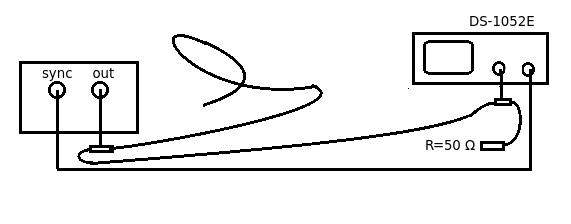
\includegraphics{Edlugie.png}
  \end{center}
\end{figure}

DG-4062 – generator krótkich impulsów
Linia zwinięta ( linia długa ) – kabel koncentryczny o impedancji charakterystycznej 50 $\Omega$, rozwarty na końcu (rezystancja dopasowująca nieskońzona) co powoduje fale odbicie impulsu.

Podsumowując - wykonywaliśmy doświadczenia na falowodach - w tym przypadku prostokątnych będących kompleksowymi zestawami pomiarówymi - i podłączonych do nich miernikach i na kablach reprezentujących linie długich.

Użyte Przyżądy:
\begin{itemize}
  \item UM 112B
  \item Miernik cyfrowy DS-1052E
  \item Oscyloskop DF4321C
  \item Miarka zwijana 40m
  \item Częstotliwościomierz U200A
\end{itemize}


\section{Wstęp teoretyczny}
\subsection{Właściwości falowe}
Klasyczne równanie falowe można zapisać w postaci:
\[ \Psi (z, t) = \Psi (z-vt)+\Psi (x+v*t) \]

Prędkość fazową definiuje się przez:
\[ v_r  =  \frac{\mathrm d z}{\mathrm d t} \]

Prędkość grupową definuje się przez:
\[ v_g = \frac{\mathrm d \omega }{\mathrm d k} \]

W przypadku fal harmonicznych:

bez dyspersji \( \omega = v_0 k \Rightarrow v_f = v_g = v_0 \).

Z dyspersją typu \( \omega ^2 = \omega _0 ^2 + v_0^2 k^2 \Rightarrow v_f v_g = v_0^2 \)

\subsection{Falowody}
Falowodem nazywamy kanał dielektryczny służący do prowadzenia w przestrzeni fal elektromagnetycznych. Właściwości falowodu zależą od jego geometrii i rodzaju materiałów konstrukcyjnych: dielektryka wypełniającego przewód i przewodzących ścianek.

W falowodach mogą rozchodzić się dwa rodzaje fal:
\begin{itemize}
\item fale poprzeczne elektrycznie TE (ang. transverse electric)
\item fale poprzeczne magnetycznie TM (ang. transverse magnetic)
\end{itemize}


Falowód prostokątny.
Istnieje wiele rozkładów pola elektrycznego i magnetycznego spełniających  równania Maxwella dla falowodu prostokątnego. Rozwiązania te nazywa się modami TEmn, występują powyżej pewnych częstotliwości granicznych.

W przypadku falowodu WR 90 (pasmo X) wymiary wynoszą a = 22,86 mm,  b = 10,16 mm.

W praktyce wykorzystuje się najczęściej mod podstawowy \( TE_{01} \) występujący powyżej częstotliwości granicznej \( f_{kr} = \frac{c} { 2a} \) ,  co odpowiada fali o długości \( \lambda _{kr} = \frac {c } { f_{kr} } = 2a\). Używanie więcej niż jednego modu na raz niezwykle komplikowałoby na przykład dekodowanie sygnałów.


Prędkość fazowa fali elektromagnetycznej w falowodzie prostokątnym jest prędkością czoła fali wzdłuż rury. Porusza się ono szybciej niż sama fala i wynosi:
\[ v_f = \frac {\omega } {k} = \lambda _f f =  \frac {v_0} { \sqrt {1 - \left( \frac { \lambda _0} { \lambda _{kr} } \right) ^2}   } < v_0 \]

Energia jest jednak przenoszona przez falę z prędkością grupową, która wynosi:
\[  v_g = \frac { d \omega } {d k} = { \sqrt {1 - \left( \frac { \lambda _0} { \lambda _{kr} } \right) ^2}   } > v_0   \]

Długość fali elektromagnetycznej \( \lambda _0 \) rozprzestrzeniającej się w falowodzie, długość fali stojącej  \( \lambda _f \) oraz krytyczna długość fali  \( \lambda _{kr} \) łączą się wzorem:

\[ \lambda _f  =  \frac {\lambda _0} { \sqrt {1 - \left( \frac { \lambda _0} { \lambda _{kr} } \right) ^2}   } \]

Występują następujące zależności pomiędzy mocami fal rozchodzących się w falowodzie:

\( P_{in} \) – moc fali padającej \\
\( P_R \) – moc fali odbitej \\
\( P_L \) – moc tracona w odbiorniku \\
\( P_{in}  = P_R + P_L \)

\subsection{Linie długie - układy o stałych rozłożonych}

W przypadku linii długich, np. gdy długości przewodu współosiowego są porównywalne z długością fali odpowiadającą częstotliwości podstawowej przekazywanego sygnału, nie możliwy jest opis zakładający, że sygnał rozchodzi się z nieskończoną prędkością. Do opisu takiej linii stosuje się układy o stałych rozłożonych. Polega to na tym, że przedstawia się linię jako bardzo krótkie segmenty przewodu, połączone ze sobą. Każdy segment charakteryzuje się przez pojemność dC i indukcyjność dL (w przypadku linii bezstratnej, do opisu linii stratnej dodatkowo dochodzi oporność dR)

\section{Wyniki pomiarów}

\subsection{Fale decymetrowe}
Wartości zmierzone lub znane: 

odległości kolejnych węzłów fali stojącej:

\begin{tabular}{|c|}
\hline 
x [mm] \\ 
\hline 
165.6\\
\hline 
314\\
\hline 
459\\
\hline 
\end{tabular} 

\( f  = 1016.31 \pm 0.02  MHz \)\\
\(a = 22.86 mm \) \\
\( U _{max}  = 0.075 \pm 0.2 V \),
\( U _{min}  = 5.4 \pm 0.2 V \)\\

Wartości wyliczone:

\( \lambda = 293.4 \pm 4 mm \)\\
\( \rho = 4.41 \pm 0.26 \) \\
\( v = 2.98 \pm 0.04 * 10^8 \frac {m} {s} \)\\
\( \Gamma = 0.63 \pm 0.02 \) \\
\( \frac {P_r} {P_{in} }  = 0.40 \pm 0.03 \) \\
\( \frac {P_r} {P_{in} } \approx 40 \% \)\\
\( \frac {P_L} {P_{in} }  = 0.60 \pm 0.03 \) \\
\( \frac {P_L} {P_{in} } \approx 60 \% \)\\


\subsection{Fale centymetrowe}
Wartości zmierzone lub znane: 

odległości kolejnych węzłów fali stojącej:

\begin{tabular}{|c|}
\hline 
x [mm] \\ 
\hline 
150 \\ 
\hline 
172 \\ 
\hline 
194 \\ 
\hline 
215 \\ 
\hline 
237 \\ 
\hline 
\end{tabular} 

\( f  = 9502 \pm 2 MHz \)\\
\(a = 22.86 mm \) \\
\( U _{max}  = 5.4 \pm 0.2 mV \),
\( U _{min}  = 5.4 \pm 0.2 mV \)\\

Wartości wyliczone:

\( \lambda = 43.5 \pm 2.9 mm \)\\
\( \rho = 7.71 \pm 2.3 \) \\
\( v = 4.13 \pm 0.27 * 10^8 \frac {m} {s} \)\\
\( \Gamma = 0.77 \pm 0.06 \) \\
\( \frac {P_r} {P_{in} }  = 0.59 \pm 0.09 \) \\
\( \frac {P_r} {P_{in} } \approx 60 \% \)\\
\( \frac {P_L} {P_{in} }  = 0.41 \pm 0.09 \) \\
\( \frac {P_L} {P_{in} } \approx 40 \% \)\\
\( \lambda _{kr}  = 0.046m \)\\
\( \lambda _{0}  = 0.032 m \)\\
\( \lambda _{f}  = 0.044 m\)\\
\( v_f = 4.14 * 10^8 \frac {m} {s} \)\\
\( v_g = 2.17 * 10^8 \frac {m} {s} \)\\

\subsection{Linie długie}
Wartości zmierzone lub znane:

Dla pierwszej serii pormiarów:

\( l_1 = 16.4 \pm 0.1 m \) \\
\( t  = 168 \pm 11 ns \) \\
\( t_x = 402 \pm 11 ns \) \\
\( c = 299792458 \frac {m} {s} \) \\

Wartości obliczone:\\
prędkość rozchodzenia się impulsu:
\( V = 0.20 \pm 0.02 \frac {m} {ns} \) \\
Długość nieznanego kabla:
\( l_2 = 39.3 \pm 2.7 m \) \\
Względna przenikalność elektryczna próżni:
\( \epsilon = 2.4 \pm 0.3 \) \\

\section{Dyskusja niepewności}
Niepewności zostały wyliczone na podstawie instrukcji dołączonych do przyrządów pomiarowych oraz zasad propagacji niepewności.

Dla przykładu kilka źródeł niepewności w pomiarach i ich wielkości:

\begin {itemize}
\item w pomiarze długości fali w części pierwszej i drugiej mieliśmy do czynienia z mierzeniem długości przyrządem o podziałce milimetrowej z noniuszem, który pozwalał na dokładniejszy odczyt, ale którego nie używaliśmy ze względu na to, że ciężko było dokładnie znaleźć węzły. Jako niepewność pojedyńczego takiego pomiaru przyjęliśmy 2 mm.

\item używając do pomiaru napięcia miernika UM 112 B z instrukcji odczytaliśmy klasę przyrządu i znając zakres na jakim dokonywaliśmy pomiary, obliczyliśmy niepewności. 

\item podczas pomiaru czasu na DS-10552E również stosowaliśmy się do uwag producenta.
$$ \Delta t = (odstęp \ próbek) + 50\cdot 10^{-6} \cdot  odczyt + 0.5 ns = (10+50\cdot 10^{-6}\cdot 168 +0.5)ns = 10.6ns  $$ 

\item przy pomiarze napiecia Oscyloskopem DF4321C, niepewność przyjęta przez nas to najmniejsza podziałka, czyli $1/5$ zakresu na jakim dokonywaliśmy pomiaru. 

\item niepewności wyznaczanych przez nas watrości były liczone poprzez sumowanie pod piewiastkiem kwadratów pochodnych danych przyczynków do błedu przemnożenych przez niepewność tych przyczynków. Czyli na przykład ( już po przekształceniach): 
%$$ \Delta \rho = \rho \cdot \sqrt{ \left( \frac {\Delta U_{max}}{U_{max}} \right) ^2 + \left (\frac { \Delta U_{min}}{U_{min} \right) ^2 } $$

$$ \Delta \rho =\rho \cdot \sqrt { \left( \frac {\Delta U_{max}} {U_{max}} \right)^2 + \left( \frac {\Delta U_{min}} {U_{min}} \right)^2 } $$
\end{itemize}


Wszystkie obliczone i zmierzone wartości w tym sprawozdaniu mają policzone niepewności pomiarowe i zamieszczone obok wartości, jeśli było możliwe ich obliczenie. Przykładem wartości bez niepewności jest jeden z parametrów falowodu: a, który został podany nam przez prowadzącego.

Niepewności pomiarowe w większości przypadków nie były szczególnie duże, wynosiły mniej niż 10\% wartości.

Jedną z największych niepewności spośród wyliczonych przez nas wartości ma:
\( \rho = 7.71 \pm 2.2 \) (pomiar decymetrowy) \\
która wynosi \( \approx 29 \% \).

To bardzo duża niepewność, ale bardzo łatwo wyśledzić jej źródło:
niepewność pomiaru napięcia minimalnego na oscyloskopie:
\( U _{min}  = 5.4 \pm 0.2 mV \)\\


\section{Wnioski}

\subsection{Fale decymetrowe}
\begin{itemize}
  \item wyznaczona przez nas prędkość fali elektromagnetycznej jest większa od prędkości światła w próżni
  \item  wartość współczynnika \( \Gamma \) wskazuje na niedopasowanie
\end{itemize}
\subsection{Fale centymetrowe}

\begin{itemize}
  \item prędkość fali rozchodzącej się w falowodzie jest w ramach niepewności pomiarowych równa prędkości światła
  
  \item wartość współczynnika odbicia \( \Gamma \) wskazuje, ze nie pracowaliśmy w stanie pełnego dopasowania. Jest to w pełni zrozumiałe, bo przed jego zmierzeniem użyliśmy stroików do uzyskania takiego stanu.
  
  \item badane fale centymetrowe należą do pasma mikrofal
\end{itemize}

\subsection{Linie długie}

\begin{itemize}
  \item metoda wykorzystywana przy pomiarze nieznanej długości może być skutecznie stosowana do znajdowania uszkodzeń kabli koncentrycznych
  \item niepewność pomiarowa długości kabla wynika głównie z niedokładności pomiary czasu
  \item wnioskujemy na podstawie wyznaczonej wartości przenikalności elektrycznej względnej izolatora, ze może on być wykonany z polietylenu ( \(\epsilon \approx 2,6 \) ).
\end{itemize}

\subsection {Podsumowanie}
Pomiary zostały wykonane wystarczająco dokładnie, by niepewności pomiarowe nie przyjęły zbyt dużych wartości uniemożliwiających rzeczową ocenę wyników.

Wyniki pomiarów pokrywają się z naszymi oczekiwaniami i wyliczeniami teoretycznymi.
\end{document}
